\documentclass[12pt]{article}

\usepackage{cls}
\usepackage{tipa}
\usepackage{enumerate}
\title{Resistance to phonetic change in York, Northern England}
\author{Daniel Lawrence}
\organization{The University of Edinburgh}

\begin{document}

\maketitle

\section{Introduction}

Research into phonological changes of the past century has yielded a set of strong generalizations regarding vocalic changes, which appear to apply across varieties of English. One example of such a generalization is the tendency for historically back vowels to move to the front of the vowel space -- Labov's (1994) `Principle III' of chain shifting. Where back vowel fronting is attested, it appears to exhibit a number of recurrent patterns in terms of a) the relative timing of the changes, b) their phonological patterning, and c) the phonetic relationship between the vowels involved. The fact that this change exhibits such striking similarities across dialects implies that it may reflect some underlying constraints on the organization of vowel systems and the processes by which those systems may change. The present paper extends research in this area by presenting evidence of the fronting of the back upgliding vowels /o/ and /u/ in a variety of northern British English, with a view to testing whether previous generalizations regarding these changes apply in this community.

\subsection{Previous work on /u/ and /o/ fronting}

The fronting of /o/ and /u/  has been documented extensively across the United States (e.g. Labov et al., 2006, Baranowski, 2008; Hall-Lew, 2009), Australia (Cox, 1999) and New Zealand (Easton \& Bauer, 2000), as well as in varieties of British English (Jansen, 2010, Kerswill \& Williams, 2000 Watt \& Tillotson, 2001). As well as being a common pattern of change, the fronting of back vowels seems to possess a number of recurrent properties, the investigation of which forms the focus of this paper. These generalizations are as follows:

\begin{enumerate}
\item{Back vowel fronting has its primary source in patterns of coarticulatory variation, the effects of which decrease over time.}
\item{/o/ fronting occurs only in dialects which also front /u/.}
\item{Where both vowels undergo fronting, /u/ fronting precedes /o/ fronting temporally.}
\item{In varieties where both vowels undergo fronting, the nucleus of \textipa{/u/} remains more advanced in F2 space than that of \textipa{/o/}.}
\end{enumerate}

The first of these generalizations refers to the fact that back vowels are fronted in post-alveolar contexts as a consequence of consonant-on-vowel coarticulation. Change in these vowels tends to involve productions in non-fronting contexts gradually moving forward, while productions in conditioning environments remain relatively constant. This pattern, reported in e.g. Durian, (2014); Harrington et al., (2006) and Hall-Lew (2011), can be taken as evidence of an internal pressure in favour of back-vowel fronting, perhaps due to learners' reanalysis of fronted allophones as production targets (e.g. Ohala, 1994; Harrington et al., 2006) and/or the articulatory cost of maintaining a category with widely separated phonetic variants (Harrington et al., 2011). Regardless of the psychological or physiological explanation of this pattern, it's prevalance implies that coarticulatory processes provide a reasonable source for diachronic fronting, meaning that this change does not necessarily involve geographical diffusion, as has sometimes been argued.

The second generalization is demonstrated very clearly in Labov, Ash and Boberg's (2005) \textit{Atlas of North American English}. Surveying the relationship between /o/ and /u/ fronting In North America, they demonstrate that North American dialects of English can be divided into three groups -- those that front /u/ alone, those that front both /u/ and /o/, and those that front neither. In no cases do they find a variety where /o/ fronts in the absence of the fronting of /u/. This observation has also been used to motivate arguments regarding the temporal relationship between change in the two vowels (point 3) above -- in Labov's (1994) model of chain-shifting, /u/ fronting is said to occur prior to /o/ fronting, triggering the raising of the latter to the position of the former. Furthermore, Labov observes there is evidence of a robust internal relationship between the two vowels, such that /u/ is always more advanced in the vowel space when both varieties front. 

While these patterns are well-attested for North American dialects, and to some extent in RP (Harrington, 2007, 2008), there is some debate as to whether northern dialects of British English are exceptional with regard to these patterns. For example, it has been claimed that \textipa{/o/} fronting occurs in the absence of \textipa{/u/} fronting in Bradford, West Yorkshire (Watt \& Tillotson, 2001), as well as in Newcastle (Watt, 2000). Haddican et al.`s (2013) study of York speech, which provides the impetus for the present work, suggests that northern British varieties may partially contradict previous generalizations due to the social indexing of dynamic vowel variation in the UK. The variable diphthongization of \text{/o/} is widely cited as a key shibboleth of northern/southern regional identity in Britain. It is thus reasonable to expect, as Haddican et al. (2013) claim, that patterns of resistance to internally-motivated change might be observed in northern England, reflecting the social values associated with dynamic characteristics of the competing forms.

\section{Data \& Methods}

\subsection{Data}

Data are taken from a corpus of production data collected from 52 individuals born between 1930 and 2000. Speakers were recruited using convenience sampling, as is typical in variationist sociolinguistic work. Table 1 provides the speakers' basic demographic information.

\vspace*{6pt}
\begin{table}[htbp]
\centering
\begin{tabular}{l|l|l}
Birth year&Female & Male \\
1935-1960 &7 &5\\
 1961-1980& 8 & 11\\
1981-2000& 10 &11\\
\end{tabular}
\caption{Characteristics of the speaker sample}
\end{table}
\vspace*{6pt}

The data include a) a 100-item wordlist, including 15 tokens of each vowel in a range of phonetic environments plus fillers; b) a map task (Anderson et al., 1991) using a selection of words from the word list and c) a sociolinguistic interview, including a range of questions relevant to the speakers' social background and identity with regard to York and the north of England. 

\subsection{Measurement}

Vowels were segmented from the first to the last glottal pulse visible in the spectrogram, and measurements of F1, F2 and F3 were taken at 20 equidistant points along the vowel trajectory. The present analysis will focus on F2 trajectories, which provide a relatively reliable reflection of the degree of fronting. Measurements were normalized using the modified Watt \& Fabricius normalization method (Watt \& Fabricius, 2002), using the mean midpoint values of \textipa{/A/} and \textsc{/i/}, measured from 4 tokens per vowel per speaker, as reference points. The formant values provided in the present analyses are of the form $F^n/S (F^n)$, i.e. the ratio of the measured frequency in Hz to the centroid frequency of that formant for the speaker being analyzed.

\subsection{Statistical analysis}

Typical sociophonetic studies have relied on the analysis of single points of the vowel trajectory (either at a fixed percentage of the token, or based on the analyst's identification of a `steady-state' target), or summary measures of trajectory length (e.g. ). The limitation of these approaches is that they may miss crucial aspects of fine-grained temporal variation in vowel realizations. In order to avoid these pitfalls, the results presented in the following sections use the statistical technique of \textit{Generalized Additive Modeling}, which allow vowel tokens to be summarized as smooth functions of time. Winter \& Wieling (2016) give a concise summary of the application of such models to time-varying linguistic data. Their key relevance of such models to the present study is that they allow the analyst to capture potentially non-linear changes in the dynamic properties of vowels, without enforcing any apriori assumptions about the shape of vowel trajectory and trajectory of change. The models presented in this paper predict normalized F2 as a function of time, plus the variables listed below:

\vspace*{6pt}
\begin{table}[!htbp]
\centering
\begin{tabular}{l|l}
Variable&Form \\
Phonetic environment & /u/: Tuw Juw Kuw uwL uw\\&/o/: Tow Kow ow owN owL\\
Log duration& Continuous \\
Speaker year of birth& Continuous (1935-2000)\\
Speaker gender& M/F \\
Speaker mobility index & (Higher/Lower) \\
Speaker regional identity index& (Higher/Lower) \\
\end{tabular}
\caption{Variables tested}
\end{table}
\vspace*{6pt}

The phonetic environments coded represent three places of articulation of the preceding consonant -- coronal contexts excluding nasals and /j/ (\textit{Tuw/Tow}), postvelar contexts excluding nasals (\textit{Kuw/Kow}) and all other contexts (\textit{ow/uw}). For /u/, Seperate codes were included for preceding /j/, known to heavily favour fronting (\textit{Juw}), and following /l/, known to heavily inhibit it (\textit{uwL}). Similarly, seperate categories were coded for /o/ tokens followed by a nasal (\textit{owN}), and those followed by /l/ (\textit{owL}).

\vspace*{6pt}
\begin{table}[!htbp]
\centering
\begin{tabular}{l|l|l}
Vowel&Variant&Criteria \\
/u/&Tuw & Preceding /j/\\
&Tuw & Preceding coronal\\
&Kuw & Preceding velar\\
&uwL & Following /l/\\
&uw & All other contexts \\
/o/&Tow & Preceding coronal\\
&Kow & Preceding velar\\
&Kow & Following /l/\\
&Kow & Following nasal\\
&ow & All other contexts
\end{tabular}
\caption{Coding criteria}
\end{table}
\vspace*{6pt}

The baseline models included constant terms for linguistic factors and their smooth interactions with time. Random smooths were included for each speaker, allowing the model to account for individual variation in vowel production.
The influence of non-linguistic factors was tested by performing a Chi-square test on models including those factors and ones with only linguistic factors. Table three describes the predictors identified as significant for each vowel:

[Table 3: model selection]
\section{Results}
\subsection{Evidence of \textipa{/o/} and \textipa{/u/} fronting in York}
Figure 1 visualizes the main effect of speaker year of birth on the second formant of \textipa{/o/} and \textipa{/u/}. At this stage, the analysis will focus on estimates taken at the vowel midpoint (50\%) -- see section 6 for a detailed discussion of the role of dynamic variation. The results demonstrate that the F2 midpoint of both vowels is reliably higher with increasing speaker year of birth, providing apparent-time evidence that both vowels have undergone fronting over the past $~$60 years. Change in \textipa{/u/} appears to have proceeded in a slightly more regular fashion that change in \textipa{/o/}, evidenced in the slightly tighter clustering of speaker means around the model predictions in Figure 1. The smooth functions estimated by the GAM analysis are roughly S-shaped, consistent with established findings on the temporal dynamics of linguistic change (e.g. Labov, xxxx). Also noteworthy is that change in \textipa{/u/} appears to have been much more radical than change in \textipa{/o/}, with change in \textipa{/u/} resulting in an increase of around .5 normalized units versus around .2 in \textipa{/o/}. 
\begin{figure}[!htbp]
\centering
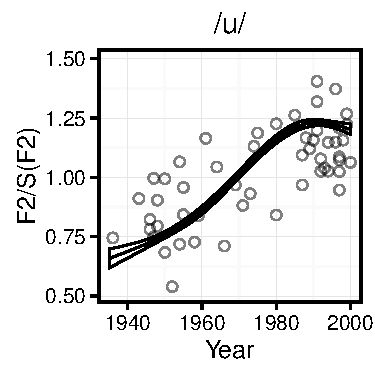
\includegraphics{uwchange}
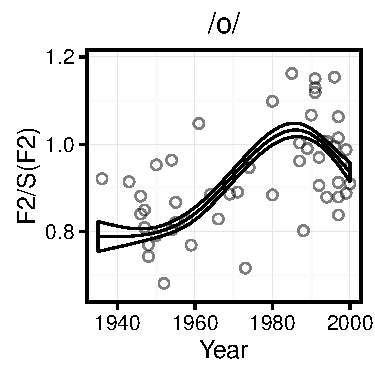
\includegraphics{owchange}
\caption{Evidence of \textipa{/o/} and \textipa{/u/} fronting}
\end{figure}

\subsection{The coarticulatory basis of \textipa{/u/} and \textipa{/o/} fronting}

The first generalization to be tested regards the proposal that coarticulatory variation provides the primary source for back vowel fronting. Under this proposal, it would be expected that the oldest speakers in the sample would demonstrate a wide range of variation in /u/ and /o/ conditioned by phonetic environment. Change would be expected to be most vigorous in those forms \textit{least} subject to coarticulatory fronting, with little or no change predicted for the \textit{most} conditioning environments. As a result, the effect of coarticulatory variation would be predicted to decrease with speaker year of birth, reflecting the generalization of fronted targets across environments. 
\begin{figure}[!htbp]
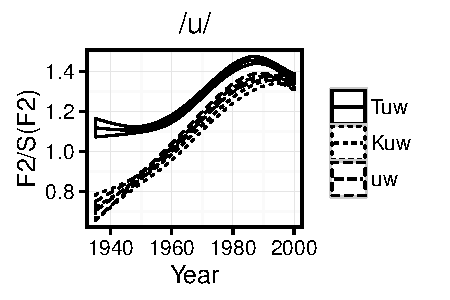
\includegraphics{uwphoneticconditioning}
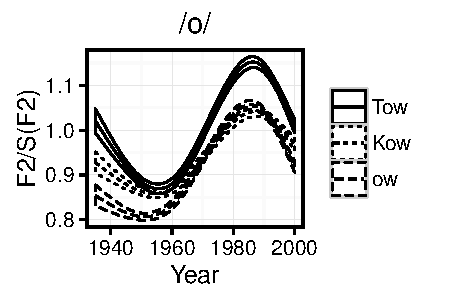
\includegraphics{owphoneticconditioning}
\caption{Changes in the phonetic conditioning of /o/ and /u/ fronting.}
\end{figure}

Figure x demonstrates the role of coarticulation in conditioning back vowel fronting in this variety, comparing the effect of preceding coronals and velars vs all other preceding contexts over time. Both vowels show some evidence of a reduction of coarticulatory effects over time, although this pattern is most noticeable for /u/. For the oldest speakers in the sample, /u/ is produced with a phonetically fronted variant following a coronal consonant (e.g. in \textit{two}), and has a back variant in all other contexts. The change takes place primarily in the non-phonetically fronting contexts, meaning that the youngest speakers in the sample produce forms such as \textit{food} and \textit{noon} with the fronted variant which was previously restricted to postcoronal environments. This pattern is less clear in the case of /o/. Although there appears to be a weaker distinction between Kow and ow contexts among speakers born after $~$1960, there is no evidence of the rapid re-alignment of allophones seen in /u/ fronting. Taken together, these results demonstrate that back vowel fronting in York adheres to the first generalization discussed in the introduction of this paper. As has been reported in other varieties of English, the coarticulatory fronting of the back vowels appears to provide a source for diachronic change. The clearest evidence for this comes from change in /u/, where the contexts demonstrating the strongest coarticulatory bias toward fronting show a smaller and less vigorous change in comparison to contexts which have no such bias. 

\subsection{The relationship between /u/ and /o/}
The second generalization to be discussed regards the cross-dialectal relationship between /o/ and /u/. The fact that both /u/ and /o/ appear to have undergone fronting confirms that this variety is not exceptional with regard to the generalization that /o/ fronting tends occur only in varieties which also front /u/. Examining estimates of the relative timing of change in the two vowels sheds further light on this relationship, and speaks to the third generalization discussed in the introduction. The panels in figure x show the estimated trajectories of change for both vowels (left-hand panel), as well as the estimated change in F2 (right hand panel). 


\begin{figure}
\centering
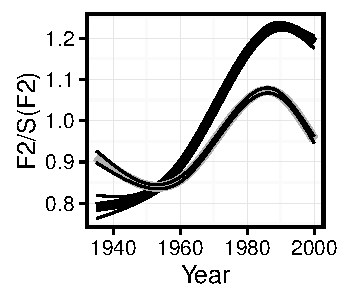
\includegraphics{owuwparallel.pdf}
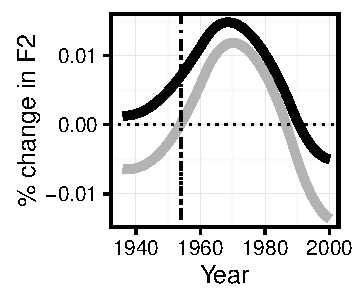
\includegraphics{owuwparallelROC.pdf}
\caption{The temporal relationship of /o/ and /u/ fronting.}
\end{figure}

While our faith in these estimates should be balanced against the relatively small size of the present sample, a number of observations can be made. Firstly, there is clear evidence that change in /u/ began before change in /o/; in fact, there appears to have been a lag of around 20 years between the onset of change in the two vowels. /u/ fronting was already in progress for speakers born 1940, while change in /o/ began in the speech of those born around the 1950s, visible where the /o/ curve crosses zero in the right-hand panel. A second observation, again consistent with previous findings, is that the rate of change in /o/ remains lower across the trajectories of change. A third observation involves the relative position of the two vowels in F2 space, and its relationship with the timing of change in /o/. Note that, for speakers born around 1940, the nucleus of /o/ is reliably in advance of that of /u/. As /u/ begins to front, its F2 target begins to approach that of /o/, and the point at which /o/ fronting begins is roughly the point at which the two vowels are parallel in F2 space. From that point on, while both /u/ and /o/ undergo fronting, the relative position of the two vowels appears to be preserved, such that the nucleus of /u/ remains reliably retracted in relation to /o/. 

The robustness of this relationship between /o/ and /u/ is demonstrated in Figure y, which plots the within-speaker relationship between the nuclei of the two vowels.

\begin{figure}
\centering
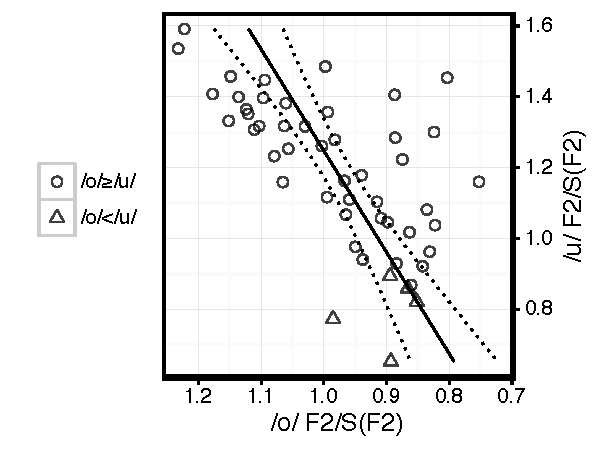
\includegraphics{owuwcorrelation.pdf}
\caption{Within-speaker relationship between /o/ and /u/.}
\end{figure}

In only four cases (represented by triangles above) do speakers show evidence of an /o/ nucleus equal to or in advance of /u/; consistent with the trajectories in figure x, these are all speakers born before the onset of /o/ fronting. These findings suggest that York speech conforms to the fourth generalization discussed in the introduction of this paper -- in varieties where both vowels front, the onset of /o/ is said to remain more retracted than /u/. Interestingly, the data suggest that while this is true for all speakers born after 1960 (the approximate onset of /o/ fronting), it is not the case for those born before that date. The implications of this will be discussed in section x.

Figure x provides a further observation of relevance, this time with regard to the claim that /o/ fronting only occurs in varieties which also front /u/. While the fact that York speech conforms to this generalization was trivially confirmed earlier in this section, considering the within-speaker relationship between the two vowels reveals that the cross-dialectal pattern is not only true when comparing varieties, but also when comparing individuals within a single variety.  While there is a clear correlation between an individuals' degree of /o/ fronting and their degree of /u/ fronting, this correlation is driven by the lack of data points in the bottom-right hand corner of the plot. While a number of speakers retain back /o/ and back /u/ (bottom, right-hand corner); some front only /u/ (top, right-hand corner), and some front both /o/ and /u/ (top, left-hand corner), few, if any speakers front /o/ without participating in /u/ fronting. This is exactly the same pattern reported cross-dialectally, here strikingly replicated within a single community. This provides convincing evidence that the phonetic relationship between /o/ and /u/ does not simply reflect historical accident -- rather, it may reflect some general bias in favor of preserving a vowel space with particular internal relationships.

\section{The internal motivation for /o/ and /u/ fronting}
To summarize the evidence presented so far, the data provide robust evidence of the fronting of /o/ and /u/ over the past 60 years in York speech. Change in these vowels is consistent with previous accounts of similar changes across varieties of English, in a number of ways:

\begin{itemize}
\item{The source of diachronic /u/ fronting appears to be related to synchronic consonant- on-vowel coarticulation, the effects of which decrease over time; however, the evidence for this process is less convincing for /o/.}

\item{/u/ fronting proceeds /o/ fronting temporally, with a lag of $~$20 years.}

\item{A speakers' participation in /o/ fronting is conditional their participation in /u/ fronting -- no speaker fronts /o/ without also fronting /o/.}

\item{There appears to be a robust pressure to maintain a relationship between the nuclei of /o/ and /u/, such that the vast majority of speakers' produce /o/ with a more retracted nucleus than /u/.}
\end{itemize}

These facts allow a tentative model of the way change in the York back vowels progressed over the past 70 years to be put forward. At the beginning of the change there was a state where /u/ was the most back category in the system, and was subject to a pattern of coarticulation whereby it was strongly fronted in post-coronal contexts. During this state, the nucleus of /o/ was relatively more centralized that that of /u/. The fronting of /u/ then began to take place, with non-post-coronal allophones gradually shifting forward to meet the phonetically fronted post-coronal realizations. This fronting of /u/ triggered the fronting of /o/, which began at roughly the same time that the nucleus of /u/ advanced further forward than that of /o/. At this point, /o/ was reanalyzed as the most back category, leading to the observed tendency for speakers to maintain an /u/ nucleus in advance of /o/.

\section{Resistance to phonetic change}

The trajectory of change thus far described has an interesting consequence. For a speaker born directly after the reanalysis of /o/ as the most back category, it would seem that the realizational possibilities of /o/ are limited, given that that speaker would presumably also have a relatively back realization of /u/, and thus be under pressure to maintain a back /o/ variant. However, as change in \textipa{/u/} progresses, the realizational possibilities for \textipa{/o/} increase -- a speaker may retain a very back form or front \textipa{/o/} to the same extent that they front \textipa{/u/}. While some speakers participate in both \textipa{/u/} and \textipa{/o/} fronting, others appear to resist fronting \textipa{/o/}. This is visualized in figure x, which plots each speakers' mean normalized F2 values, with each individual's \textipa{/o/} and \textipa{/u/} joined by a dotted line. It can be seen that speakers born before 1960 have relatively little distance between the two vowels, and three speakers have a more retracted \textipa{/u/} realizations than \textipa{/o/}. After 1960, all speakers keep \textipa{/u/} in front of \textipa{/o/}, and some appear to retain a back \textipa{/o/} variant, equally or even more backed than the oldest speakers in this sample.

\begin{figure}
\centering
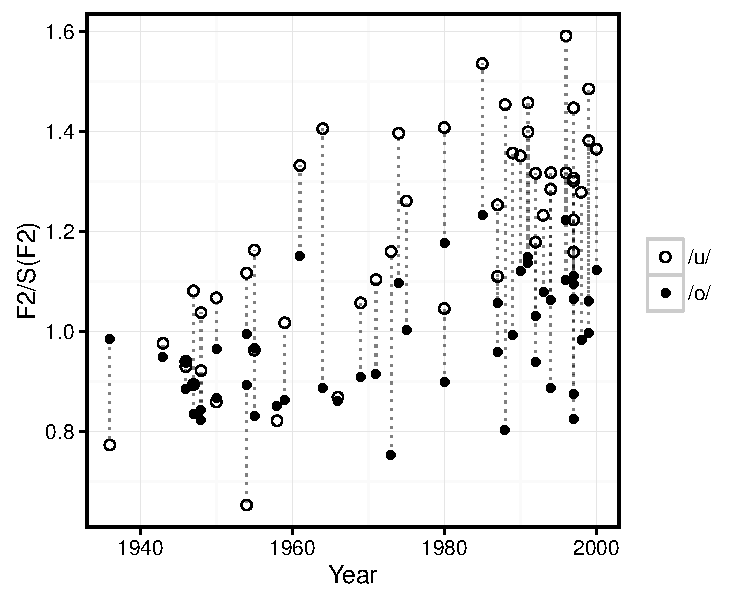
\includegraphics[scale=.75]{resistance1.pdf}
\caption{Relationship between /o/ fronting and diphthongization.}
\end{figure}

What causes this resistance to fronting among certain younger speakers? Given that the variable diphthongization of \textipa{/o/} is widely noted as a marker of regional identity, it is reasonable to predict that dynamic properties of this vowel might play a role. Exploring the relationship between fronting and diphthongization reveals and interesting pattern, demonstrated in figure x. Speakers appear to cluster into three groups in acoustic space 00 some have a back, monophthongal \textipa{/o/}; some have back, diphthongal \textipa{/o/}, and some have a fronted, diphthongal variant. Notably, there seems to be a lack of cases of fronted, diphthongal \textipa{/o/}. The speakers who resist fronting are those who retain a monophthongal variant.

\begin{figure}
\centering
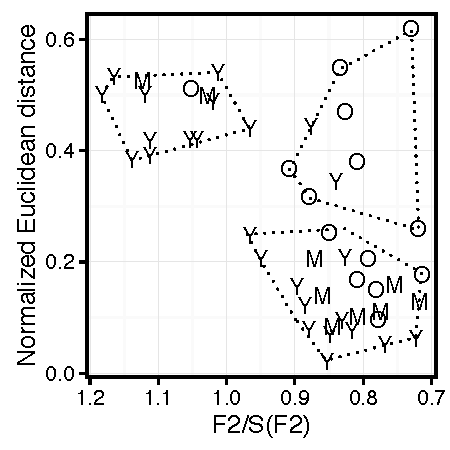
\includegraphics{ofrontingdip.pdf}
\caption{Relationship between /o/ fronting and diphthongization.}
\end{figure}

This pattern is consistent with recent findings on this community (Haddican et al., 2013), with the exception that the authors found fronted monophthongs among their middle group of speakers (born 1967-1981), in contrast to the complete absence of such forms in the present data. There are at least two possible explanations for a pattern like this. If we imagine a general pressure to front both \textipa{/o/} and \text{/u/}, then it might be proposed that speakers avoid participating in \textipa{/o/} fronting due to a stigmatization of fronted, monophthongal variants. This is similar to the phenomenon of \textit{sound change supression} mentioned in Kroch (1978) and Thomason (2016), in which the stigmatization of certain sounds leads to their loss from a particular variety. Haddican et al. (2013) develop this argument in detail, proposing that younger speakers associate monophthongal /o/ with a stigmatized, class-based stereotype, the \textit{chav}. Under this account, all speakers are subject to an internally-motivated pressure to front, but this pressure is blocked by the negative social indexing among monophthongal speakers. While there is some evidence that younger speakers indeed produce fronted, monophthongal variants when performing this stereotype, a second explanation should also be considered -- rather than this being a pattern of resistance per se, it could be that fronting is accelerated among diphthongal speakers due to the temporal-dynamic characteristics of their \textipa{/o/} productions. In other words, everyone fronts \textipa{/o/} a little, but diphthongal speakers appear to front more radically. Exploring the patterning of dynamic variation of \textipa{/o/} across speaker groups strongly suggests that this is the case. 

\begin{figure}
\centering
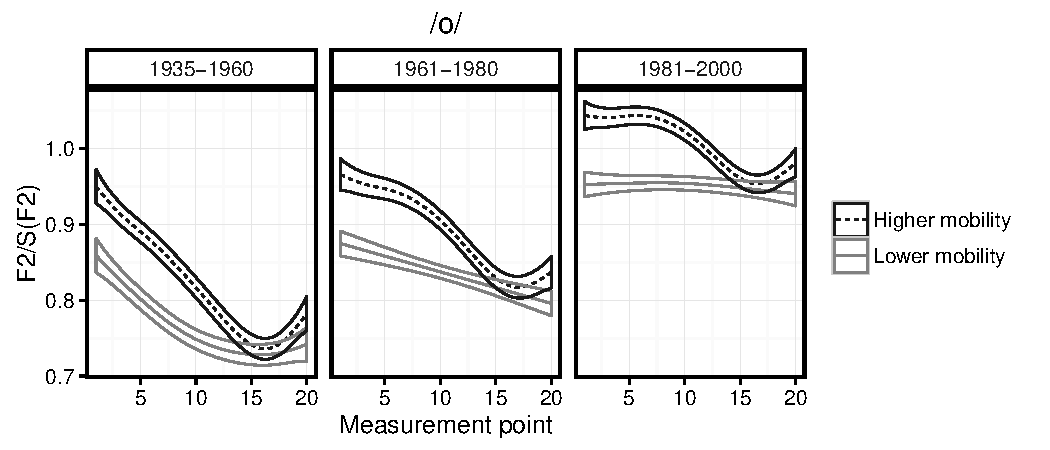
\includegraphics[scale=0.9]{owdynamicsclass.pdf}
\caption{Estimated /o/ F2 trajectory by decade and mobility group.}
\end{figure}

Figure x plots predicted contours for the high-mobility and low-mobility groups, faceted by year of birth. It is clear that for all age groups, more mobile speakers are reliably more diphthongal than less mobile speakers, presumably representing the more mobile speakers appoximating a Southern Standard British English form. Fronting appears to have two effects -- fronting among less mobile speakers involves a shift across the entire F2 trajectory, as well as fronting at the offglide. This results in an overall more monophthongal average trajectory among younger, less mobile speakers. Among more mobile speakers, fronting happens at both the vowel onset (around the seventh measurement point) and offglide, resulting in a much more curved trajectory among younger speakers. A side effect of this interaction between fronting and diphthongization is that fronting appears more advanced among the more mobile group. Overall, this suggests that the observed pattern of `resistance' may not be resistance at all -- rather, fronting may have lead the amplification of existing socially-conditioned differences in the temporal dynamics of the back vowels, leading to more mobile speakers producing more fronted, diphthongal realizations than less mobile speakers. While the account of social-indexically motivated resistance to internal pressures presented in Haddican et al. (2013) is perfectly feasible, paying attention to the fine-grained temporal details of this vowel suggests that an explanation based on the combined effects of speaker mobility and internal pressures better fit the data.

\section{Conclusion}

This paper has presented apparent-time evidence of the fronting of the back upgliding vowels over the past ~70 years in York, northern England. Its core aim was to test a set of cross-varietal generalizations regarding back vowel fronting, including their phonological patterning, relative timing, and phonetic relationship. In general, the evidence suggests that back vowel fronting in York conforms to previous generalizations, adding to the evidence that Labov's `Principle III' of vowel shifting may apply across varieties of English, and possibly reflect some general biases towards certain kinds of change occuring cross-linguistically. Investigating these generalizations suggests a number of innovative findings. Firstly, the distribution of \textipa{/u/} and \textipa{/o/} fronting across varieties of English appears to be reflected at the community level. Previous work has found that English dialects tend to either front only \textipa{/u/}, both \textipa{/u/} and \textipa{/o/}, or neither. The present findings demonstrates that speakers seem to replicate this pattern within a single community, in that very few speakers front \textipa{/o/} without participating in \textipa{/u/} fronting. A related second point regards the phonetic relationship between the two vowels -- there appears to be a robust constraint on their relative position, with each speaker's \textipa{/u/} nucleus remaining reliably fronter than that of \textipa{/o/}. Thirdly, there is some evidence that this constraint was only adopted once change in \textipa{/o/} had actuated in this community, which also happened to be the point where the nucleus of \textipa{/u/} passed that of \textipa{/o/} in F2 space. While exploring the exact process which might lead to this situation is beyond the scope of the present work, it seems that the movement of \textipa{/u/} past \textipa{/o/} initiated change in \textipa{/o/}, and also caused the reanalysis of \textipa{/o/} as the most back category in the system, leading to the observed relationship between the two vowels.

The final section of the present work explored the influence of social factors on speakers \textipa{/o/} productions. While \textipa{/u/} fronts in a relatively uniform manner, many younger speakers appear to resist fronting \textipa{/o/}. Examining the role of dynamic variation in \textipa{/o/} revealed considerable interspeaker variation. Speakers cluster into three groups -- those with a back, diphthongal variant; those with a back, monophthongal variant; and those with a fronted, diphthongal variant. Two interpretations of this pattern were discussed -- firstly, that monophthongal speakers resist fronting due to the social indexicality of fronted, monophthongal variants, as suggested by Haddican et al. (2013). This explanation was rejected in favour of an alternative -- that the advanced fronting observed among diphthongal speakers is related to the effect of fronting on diphthongal speakers' F2 contour, resulting in more fronted variants among that group. Evidence in favour of this account came from an analysis of vowel trajectories across speaker groups, which revealed that diphthongization is systematically related to speakers' mobility. Speakers who have more contact with people from outside of York are more likely to produce a diphthong, and the absolute difference between monophthongal and diphthongal speakers increases as a consequence of fronting.


\subsection{References}

Please use LSA style: name (year or (Name year). Formulations
with author names like ``\ldots\ as \namecite{Ladefoged:2003}
showed that \ldots'' are acceptable, but not ``as shown in [Ladefoged,
2003]'' or ``as shown in (Ladefoged~[6])''. See Section 4 for more on references.


\section{Format of references}

Monographs such as \namecite{Fant:1960} consist of author(s) last name(s),
initial of the first name(s), year of publication, title in italics, location of the publication, and publisher. The names of multiple authors are separated by commas listed in the 
sequence last name, comma, initial(s) of the first name(s) (cf.\ the examples~\citeboth{Beattie/etal:1982}, \citeboth{Peterson/Barney:1952}). 

Contributions to volumes, e.g.~\namecite{Stevens:1999}, follow the
convention that the title of the volume is in italics, but not the
title of the contribution. Book editors should appear after the book title, 
followed by page numbers, place of publication, and publisher.

Journal articles should be handled in the same way as contributions to
volumes, except that the title of the journal is in italics and
the editors are not listed. Longer names of well-known journals can be
abbreviated (e.g.~\citeboth{Peterson/Barney:1952}).

Articles in conference proceedings such as \namecite{Ladefoged:2003} are
referenced in the same way as journal articles.  The word
\textit{proceedings} can be abbreviated and the location should be
mentioned after the name of the conference. Here, abbreviations of
well-known conferences are possible.

\bibliographystyle{clslike}
\bibliography{cls}

\end{document}

